\documentclass[10pt,conference]{IEEEtran}
\IEEEoverridecommandlockouts

\usepackage[T1]{fontenc}
\usepackage{amsmath,amssymb}
\usepackage{newtxtext,newtxmath}
\usepackage{cite}
\usepackage{graphicx}
\usepackage{booktabs}
\usepackage[hidelinks]{hyperref}
\usepackage{url}
\usepackage{balance}

\graphicspath{{../dolap_dataset/figures/}}

\begin{document}

\title{A Longitudinal Corpus of Data-Transformation\\Lineage Reconstructed from dbt Project Histories}

\author{\IEEEauthorblockN{Dineshkumar Malempati Hari}
\IEEEauthorblockA{\textit{Independent Researcher} \\
\texttt{mhdk.dinesh@gmail.com} \\
\href{https://orcid.org/0009-0003-1036-9477}{orcid.org/0009-0003-1036-9477}}}

\maketitle

\begin{abstract}
Production tooling emits data-transformation lineage continuously and almost
never publishes it. OpenLineage, Marquez and Egeria all ship dbt integrations,
and none of them releases a corpus, because the events originate inside private
warehouses. Reconstruction from repository history is therefore the only
available route to a public longitudinal record of how transformation graphs
change. I release 3{,}586 monthly lineage snapshots of 154 public dbt projects,
453{,}108 nodes and 503{,}925 edges over 566 cumulative project-years and a
decade of wall-clock time, recovered by parsing \texttt{ref()} declarations out
of the git object database without executing dbt and without a warehouse
connection. The corpus is a systematic sample of a documented frame of 3{,}718
candidates rather than a census of public dbt, and the screen that produced it
ships with the data. Every edge carries the parse mode that found it, so a
stricter reader reconstructs a stricter graph exactly. Three findings that
nothing public could previously test are reported, the strongest being that the
staging, intermediate and mart taxonomy does not describe the median public dbt
project at all.
\end{abstract}

\begin{IEEEkeywords}
data lineage, dbt, analytics engineering, mining software repositories, dataset
\end{IEEEkeywords}

\section{Introduction}

The literature on data-transformation lineage is not thin. It is absent. A dblp
query for \emph{dbt} or \emph{data build tool} returns no matching publication,
no matching venue and no matching author. The Directory of MSR
Datasets~\cite{msrdirectory} indexes 196 datasets and not one of them concerns
lineage, dbt, SQL transformation, ETL or warehouse schema, in a directory that
already carries GitHub Actions workflow histories~\cite{cardoen2024} and
Terraform programs~\cite{terrads2025}. Declarative infrastructure has been
mined. The layer that actually moves the data has not.

dbt is the object worth mining, and one design decision is why. A dbt model is a
SQL file whose upstream dependencies are declared through a \texttt{ref()}
function rather than inferred from the SQL text. The dependency graph is
therefore recoverable by reading the files, with no parser for a warehouse SQL
dialect and no semantic analysis of joins. I exploit exactly that property and
nothing else.

No corpus exists today because the instrumentation that would produce one is
private by construction. OpenLineage defines an open standard for run-time
lineage events and ships a dbt wrapper~\cite{openlineage}; Marquez is its
reference backend and Egeria is a second one. All three are mature, all three
are adopted, and the events they carry describe a company's own warehouse, so
none of them can publish a historical record. Repository reconstruction is the
remaining route.

That route is not a parser invoked $N$ times, and I want the distinction visible
here rather than defended in Section~\ref{sec:limits}. The frame is a
three-stratum harvest over 3{,}718 candidates, with star-band and size-band
partitioning used to work around GitHub's 1{,}000-result pagination cap. The
screen is documented condition by condition and every decision is released.
Fidelity is measured per repository against a second parse rather than asserted.
The extraction reads trees and blobs straight out of the object database instead
of checking out each commit, which is what makes a 56-snapshot history cheap
enough to run 631 times.

My contributions are four. First, the corpus, 3{,}586 lineage snapshots of 154
projects with a graph and 15 descriptors at each. Second, the extraction tool,
unit tested and separately citable. Third, a characterization establishing that
the canonical dbt layer taxonomy fails to describe the median public project.
Fourth, the released artifact, its documented frame and its manifest of 626
checksummed files.

\section{The corpus}

\subsection{Sampling frame and yield}
\label{sec:frame}

The frame is a systematic sample of a documented population, not a census of
public dbt, and the reason is a platform limit. GitHub code search reports
5{,}340 hits for \texttt{filename:dbt\_project.yml} and paginates at 1{,}000, so
I partitioned the query into twelve repository-size bands and recovered 2{,}207
of those hits. Three strata were unioned and deduplicated. S1 is the 20 entries
of a widely used curated list, which a reader reaches for first and which yields
two projects. S2 is repository
search over five dbt topics, each split into ten star bands for the same reason.
S3 is the code search above. The union is 3{,}718 candidates and it is released
in full.

Screening removed only candidates for which no monthly series can exist. Fewer
than 40 commits on the default branch removed 2{,}275, fewer than 12 months
between creation and last push removed 811, and unresolvable metadata removed
one. What a repository looks like at HEAD was recorded and never used to
exclude, because a HEAD test is blind to the adoption-and-abandonment lifecycle
a longitudinal corpus should contain. One project in the release used dbt for
two years, stopped, and still contributes 27 snapshots.

The 631 survivors were cloned and extracted, and membership was decided from the
extraction. A project enters the corpus on three conditions, at least 12 monthly
snapshots, a peak of at least 10 nodes, and one resolvable
\texttt{dbt\_project.yml} somewhere in its history. That yields 154 projects.
The 12-snapshot floor is an elbow rather than a preference, since relaxing it to
six adds 74 projects and only 609 snapshots, eight apiece, while raising it to
eighteen costs 62 projects and 870 snapshots. Both alternatives are tabulated in
the release. The 154 span 2016-07-27 to 2026-08-04.

Two labels partition the corpus and both ship as columns. Composition separates
55 analytics estates from 95 reusable packages and 4 demos by ordered rules, of
which the independent one, shipping an \texttt{integration\_tests} project,
reaches 0.857 accuracy alone on a hand-labelled sample of 28. The naming rule
after it is partly circular on that sample and the release says so. Connectivity
was tried as a classifier and rejected at 0.643.

I also split the corpus into 33 \texttt{core} and 121 \texttt{extended}
projects. A package can clear the inclusion criteria with fifty model files and three
edges among them, and on a graph that sparse a connectivity descriptor describes
a handful of nodes while $N$ reports fifty. Core requires
24 snapshots, a peak of 25 nodes and a median giant component of at least half
of $N$. Neither tier is filtered out and both are real measurements.

\subsection{Extraction}

Commits touching a declared model path are listed oldest first under
first-parent traversal. The history is cut into rolling 30-day windows anchored
on the first such commit, and the last commit in each window becomes a snapshot,
so a quiet month yields nothing and a busy month yields one. At the sampled
commit the extractor reads every \texttt{.sql} file under the resolved
\texttt{model-paths}, skipping macros, tests, snapshots and vendored packages. A
node is the filename stem, as in dbt itself, since model names are globally
unique within a project. An edge runs from \texttt{ref('a')} to the
model whose file contains it, and only when \texttt{a} resolves to another model
in the same snapshot.

Nothing is checked out. Trees come from \texttt{git ls-tree} and file contents
from a single \texttt{git cat-file -{}-batch} process per snapshot, so the
worktree is never mutated and one clone can be read concurrently. Cal-ITP's 53
snapshots take under 30 seconds on one core, against minutes for the
checkout-per-snapshot predecessor, and a regression test asserts that HEAD, the
porcelain status and the checked-out branch are unchanged after a run.

Comments are stripped before matching, \texttt{-{}-}, \texttt{/* */} and
\texttt{\{\# \#\}} alike. Without that step a commented-out reference becomes an
edge, and across the corpus 3{,}963 such phantom edges were discarded.

\begin{table*}[t]
\centering
\caption{Schema of \texttt{snapshots.csv}, the primary table. Primary key is
(\texttt{project\_id}, \texttt{sha}). The four layer counts sum to $N$ at every
snapshot. \texttt{schema.json} in the release carries the same dictionary for
every other file.}
\label{tab:schema}
\scriptsize
\setlength{\tabcolsep}{3.5pt}
\begin{tabular}{@{}llp{0.205\linewidth}@{\hspace{8pt}}llp{0.185\linewidth}@{}}
\toprule
Field & Type & Meaning & Field & Type & Meaning \\
\midrule
\texttt{project\_id} & string & owner and repo, double underscore & \texttt{giant\_component\_frac} & float (0,1] & largest component over $N$ \\
\texttt{date} & datetime & git author timestamp & \texttt{isolated\_frac} & float [0,1] & models with no edge \\
\texttt{sha} & 40 hex & commit the snapshot was read at & \texttt{n\_staging} & integer & models named as staging \\
\texttt{commit\_msg} & string & subject line, 120 chars & \texttt{n\_intermediate} & integer & models named as intermediate \\
\texttt{N} & integer & resolved dbt models & \texttt{n\_mart} & integer & mart, fact, dimension, reporting \\
\texttt{M} & integer & model-to-model \texttt{ref()} edges & \texttt{n\_unclassified} & integer & matching no layer rule \\
\texttt{too\_small} & boolean & true when $N<5$, descriptors skipped & \texttt{n\_sql\_files} & integer & files read, before stem collapsing \\
\texttt{D1\_csi} & float [0,1] & community stability, \emph{not released} & \texttt{n\_dbt\_projects} & integer & visible \texttt{dbt\_project.yml} \\
\texttt{D1\_n\_comm} & integer & Louvain communities, \emph{not released} & \texttt{M\_strict} & integer & edges the anchored pattern finds \\
\texttt{D2\_max\_gini} & float [0,1] & max over depth of blast-radius Gini & \texttt{M\_recovered\_by\_permissive} & integer & edges only the unanchored pattern finds \\
\texttt{D3\_alg\_conn} & float $\geq 0$ & algebraic connectivity & \texttt{nodes\_touched\_by\_recovered} & integer & nodes incident to a recovered edge \\
\texttt{D3\_norm\_gap} & float [0,1] & $\lambda_2$ over $\lambda_{\max}$ & \texttt{edges\_dropped\_as\_commented\_out} & integer & phantom edges a naive parse invents \\
\texttt{D3\_fiedler\_bim} & float [0,1] & Fiedler bimodality, see \S\ref{sec:limits} & \texttt{n\_documented} & integer & models with a YAML description \\
\texttt{D4\_cycle\_rank\_norm} & float $\geq 0$ & $(M-N+C)$ over $N$ & \texttt{n\_tested} & integer & models carrying a dbt test \\
\texttt{n\_components} & integer & components of the skeleton & \texttt{doc\_rate}, \texttt{test\_rate} & float [0,1] & the two counts above over $N$ \\
\bottomrule
\end{tabular}
\end{table*}

\subsection{Storage and schema}

The release is 9.0\,MB of UTF-8 CSV and JSON across 626 files, every one of them
carrying a SHA-256 in \texttt{MANIFEST.json}. Eight artifacts matter to a reader.
\texttt{snapshots.csv} holds all 3{,}586 rows and its schema is
Table~\ref{tab:schema}. \texttt{corpus\_index.csv} is the yield table, one row
per project with span, size range, growth, tier, composition, cadence and
fidelity. \texttt{edges/<id>.csv.gz} holds every edge of
every snapshot so a reader can rebuild any graph rather than trust the scalars.
\texttt{drift\_events.csv} records the 989 consecutive-snapshot changes above
20\,\% in a descriptor. \texttt{sampling\_frame.csv} and \texttt{excluded.csv}
carry the 3{,}718 candidates and the 488 post-extraction rejections with a
reason each. \texttt{schema.json} is the machine-readable dictionary and
\texttt{MANIFEST.json} the provenance.

Provenance is pinned rather than described. \texttt{MANIFEST.json} records the
tool version, here 2.0.0, the repository URL, the default branch, the HEAD SHA at
extraction time and the SHA of every sampled commit, so any row traces back to
the exact tree it came from even after the repository moves on. Rerunning the pipeline
against live repositories will not reproduce the corpus, and I say so plainly.
Cal-ITP had 1{,}019 model-touching commits when an earlier two-project study ran
and 1{,}049 when this corpus was built.

\subsection{Parse fidelity, measured per repository}
\label{sec:fidelity}

The extractor runs two patterns. The strict one requires \texttt{\{\{}
immediately before \texttt{ref(}, so it sees only a ref that is the whole Jinja
expression. The permissive one drops the anchor and also accepts the
two-argument \texttt{ref('package','model')} form, so it sees a ref handed to a
macro such as \texttt{dbt\_utils.union\_relations} or \texttt{unpivot}. Those
sites are plain string literals and dbt resolves them, so the corpus reports the
permissive parse.

The aggregate is the number that would have misled. Across the corpus the anchor
hides 43{,}893 of 503{,}925 edges, 8.7\,\%, and quoting that alone implies a
uniform tax. The distribution says otherwise. The median project loses nothing,
99 of the 154 lose no edge at all to the anchor, the ninetieth percentile is
8.5\,\% and the worst project loses 54.4\,\%. Fidelity is a per-repository
property and \texttt{corpus\_index.csv} reports it that way. Every row in
\texttt{edges/} carries \texttt{capture\_mode}, so filtering to \texttt{strict}
reconstructs the 460{,}032 edges of the anchored parse exactly.

\section{What the corpus shows}

The characterization supports the artifact and is deliberately short.

\textbf{The canonical layer taxonomy does not describe the median public dbt
project.} Staging, intermediate and mart is the architecture dbt's own
documentation teaches. Across the 154 projects the median per-project share of
intermediate models is exactly 0.00 and the median share of mart models is
exactly 0.00. At their final snapshot, 56 projects have more unclassified models
than staging, intermediate and mart put together. Layer labels come from naming
conventions rather than dbt metadata, so a private convention reads as
unclassified. That is itself the finding. A taxonomy
nobody names in a file path is not one a tool can rely on.

\textbf{The median public dbt package is a forest.} Fig.~\ref{fig:acyclic} plots
the per-project median normalized cycle rank by composition, and the mass at
exactly zero is the point. Half of the 95 packages, 51\,\%, carry no cycle at
all in the undirected skeleton, against 24\,\% of the 55 analytics estates, with
medians of 0.000 and 0.161. The separation survives the 43{,}893-edge recovery
of \S\ref{sec:fidelity} rather than being produced by it, because the recovered
edges sit in macro-heavy estates and cannot reach the sparse packages the result
rests on.

\textbf{Growth is real but modest.} The median project ends at 4.09 times its
first-snapshot node count, and at 2.41 times its first \emph{viable} snapshot,
the latter being the honest figure because many histories start at two or three
models. Fig.~\ref{fig:growth} normalizes every trajectory to its own origin.

\textbf{The failures are a finding.} Of the 631 repositories cloned, 186
produced no usable series. Two had gone unreachable between harvest and clone.
Of the 184 with a recorded reason, 81 carry no \texttt{dbt\_project.yml} anywhere
on their first-parent history, which means GitHub's code index served me a file
that had been deleted, and 78 declare model paths to which no commit ever wrote.
A public mirror of an internal estate often publishes the project file and
withholds the SQL. Anyone sizing a dbt study from search counts should expect to
lose roughly a third of the hits this way.

\begin{figure}[t]
\centering
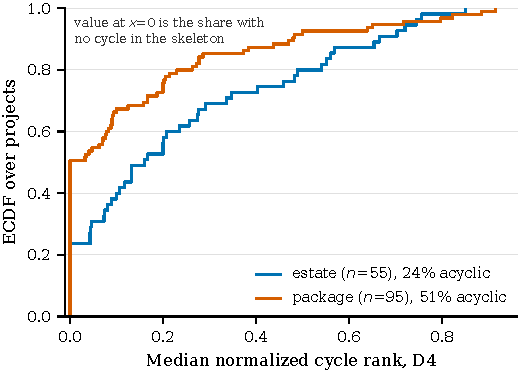
\includegraphics[width=\columnwidth]{fig4_acyclicity_by_composition.pdf}
\caption{Per-project median normalized cycle rank, by composition. The value at
$x=0$ reads directly as the share of projects with no cycle in the undirected
skeleton. Demo projects ($n=4$) are omitted as too few for an ECDF.}
\label{fig:acyclic}
\end{figure}

\begin{figure}[t]
\centering
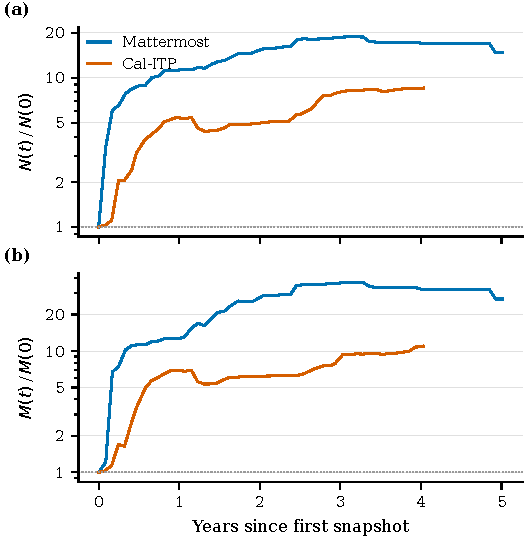
\includegraphics[width=0.86\columnwidth]{fig2_growth_normalized.pdf}
\caption{Node and edge counts normalized to each project's own first snapshot,
all 154 projects, with the corpus median and interquartile range in black. The
log ordinate compresses a range that spans three orders of magnitude.}
\label{fig:growth}
\end{figure}

\section{Related datasets}

\textbf{Schema histories.} Vassiliadis et al.~\cite{vassiliadis2023} mine 195
FOSS relational schema histories per commit without running the systems, and
their framing of the absence of public schema histories is the one I echo here.
The object separates us cleanly. They record how a storage schema changes; I
record how the transformation topology above it changes, which is a different
graph over different artifacts, and their 195 is a precedent for my 154 rather
than a comparison I need to win.

\textbf{Declarative artifact histories.} Cardoen et al.~\cite{cardoen2024}
release the commit histories of GitHub Actions workflow files and the
\texttt{gigawork} tool that extracts them, and TerraDS~\cite{terrads2025}
releases Terraform HCL programs. Mining a declarative file out of git history is
routine, and I claim none of it. This corpus does for the transformation layer
what those two do for CI and for provisioning, and the longitudinal design is
deliberately theirs.

\textbf{Static pipeline extraction.} APEX-DAG~\cite{eggers2025} extracts data
pipelines from Python ML code by static analysis, explicitly without executing
the code. Extraction without execution is therefore already claimed and I do not
repeat it. Two things differ. APEX-DAG infers
dataflow where I read an explicit declaration, and it operates on single
snapshots and releases no dataset, where the longitudinal axis and the release
are the whole of my contribution. The sentence I do claim is narrow. This is the
first publicly available longitudinal corpus of data-transformation lineage.

\textbf{Workflow execution traces.} WfCommons~\cite{coleman2022} publishes
traces of workflow runs, which is a record of execution rather than of
repository-derived topology. It also supplies the precedent that a
workflow-structure corpus of roughly 180 units is publishable.

\section{Use to date, and what to improve}

An earlier two-project version of this pipeline supported a study of whether
lineage topology proxies governance maturity. That study returned a negative
result, its correlation being carried by architectural layer rather than by
governance, and its release~\cite{hari2026} covers 106 snapshots of two estates.
This corpus supersedes it by a factor of 34 in snapshots and 77 in projects,
and it exists because two estates cannot separate a real effect from a
coincidence of two organizations. No other use has been published.

Four improvements are worth naming. Resolving \texttt{source()} and seeds from
the schema YAML beside the models would close most of the gap against a compiled
manifest. Git similarity detection would let a rename read as a rename rather
than as a birth and a death. A real \texttt{dbt compile} manifest for the subset
of projects that still build would give a ground-truth calibration set instead
of the single audited project I have. And a frame built from an event archive
would escape the pagination cap that costs me 3{,}133 code-search hits.

\section{Research opportunities}

Four questions become answerable, and nothing else public can answer them.

Do transformation DAGs stabilize the way relational schemas do? Skoulis et
al.~\cite{skoulis2015} found expansion under a perfective-maintenance brake in
open-source databases. The corpus carries 566 project-years and 989 marked drift
events, so their named shapes can be tested directly on a different artifact.

Does documentation keep pace with structure? Every snapshot carries
\texttt{doc\_rate} and \texttt{test\_rate} beside $N$. A within-project analysis
over 119 projects with a non-constant series already gives a median Spearman
$\rho$ of $-0.152$ between documentation rate and size, a weak negative worth a
proper treatment.

Does layer composition converge as independently developed estates mature? The
release makes the institutional-convergence question testable in a form that
does not depend on interviewing anybody.

And what does an abandoned dbt estate look like on the way down? Thirty-nine
projects end below their own node peak, one of them 84.6\,\% below, so a growth
multiple is not the range a graph traverses.

\section{Limitations}
\label{sec:limits}

\texttt{source()} is not resolved. An edge is emitted only when a \texttt{ref()}
argument names another model in the same snapshot, so external inputs, seeds and
cross-package references are absent, graphs fragment more than a compiled
manifest would, and node counts understate it. Measured against a real
\texttt{dbt compile} on the largest project I audited, the parse recovers 631 of
885 nodes, and the shortfall is sources and seeds.

Renames are not tracked. A model renamed between snapshots reads as one node
disappearing and another appearing, which inflates churn.

Cadence is irregular. One snapshot per 30-day window of activity is a target,
not a guarantee. The median project's own median gap is 39 days and the worst
single gap in the corpus is 1{,}686 days.

Two descriptors are unsafe and I say which. \texttt{D1\_csi} and
\texttt{D1\_n\_comm} come from Louvain, whose result depends on node insertion
order, and under twelve permutations of the same graph \texttt{D1\_csi} moves by
as much as 0.5714 against a published standard deviation of 0.123. Both are
excluded from every figure. \texttt{D3\_fiedler\_bim} is not unstable but
undefined wherever the second Laplacian eigenvalue is degenerate, since the
Fiedler vector is then not unique, and the corpus contains a 15-node component
whose $\lambda_2$ through $\lambda_6$ are separated by $4.4\times10^{-16}$.
Check the eigenvalue separation before trusting a Fiedler vector.

First-parent traversal drops parallel branches, a choice inherited from
\texttt{gigawork}~\cite{cardoen2024}. Public projects are not enterprise
estates, and \texttt{ref()} records declared dependencies, not executed ones.

Finally, path resolution can silently shrink a real estate.
\texttt{catalyst-cooperative/pudl} has 11{,}147 commits and was excluded at a
peak of 2 nodes, because the models the extractor could resolve were not the
models the project runs. Nothing in the pipeline detects that case, and a reader
comparing the corpus against a project they know should expect it.

\section{Availability}

Corpus, tool, frame and manifest are MIT licensed and archived under concept DOI
\href{https://doi.org/10.5281/zenodo.20099999}{10.5281/zenodo.20099999}, with a
\texttt{requirements.txt} and a command line per pipeline stage. Data and code
carry separate citable version DOIs.

\balance

\begin{thebibliography}{99}

\bibitem{msrdirectory}
Directory of MSR Datasets, Aristotle University of Thessaloniki. [Online].
Available: \url{https://authecesofteng.github.io/directory-msr-datasets/}.
Accessed 5 Aug. 2026, 196 datasets indexed.

\bibitem{cardoen2024}
G. Cardoen, T. Mens, and A. Decan, ``A dataset of GitHub Actions workflow
histories,'' in \emph{Proc. 21st Int. Conf. Mining Software Repositories (MSR)},
Lisbon, Portugal, 2024, pp. 677--681, doi: 10.1145/3643991.3644867.

\bibitem{terrads2025}
C. B\"{u}hler, D. Spielmann, R. Meier, and G. Salvaneschi, ``TerraDS: A dataset
for Terraform HCL programs,'' in \emph{Proc. 22nd Int. Conf. Mining Software
Repositories (MSR), Data and Tool Showcase Track}, Ottawa, Canada, 2025,
doi: 10.1109/MSR66628.2025.00061.

\bibitem{openlineage}
OpenLineage, ``dbt integration.'' [Online]. Available:
\url{https://openlineage.io/docs/integrations/dbt/}. Accessed 5 Aug. 2026.

\bibitem{vassiliadis2023}
P. Vassiliadis, F. Shehaj, G. Kalampokis, and A. V. Zarras, ``Joint source and
schema evolution: Insights from a study of 195 FOSS projects,'' in \emph{Proc.
26th Int. Conf. Extending Database Technology (EDBT)}, Ioannina, Greece, 2023,
pp. 27--39, doi: 10.48786/edbt.2023.03.

\bibitem{eggers2025}
S. Eggers, N. \.{Z}ukowska, and Z. Abedjan, ``APEX-DAG: Library and language
independent pipeline extraction,'' \emph{Proc. VLDB Endowment}, vol. 18, no. 12,
pp. 5375--5378, 2025.

\bibitem{coleman2022}
T. Coleman, H. Casanova, L. Pottier, M. Kaushik, E. Deelman, and R. Ferreira da
Silva, ``WfCommons: A framework for enabling scientific workflow research and
development,'' \emph{Future Generation Computer Systems}, vol. 128,
pp. 16--27, 2022, doi: 10.1016/j.future.2021.09.043.

\bibitem{hari2026}
D. Malempati Hari, ``Multiscale governance descriptors for data lineage graphs,''
Zenodo, v1.0.0, 2026, doi: 10.5281/zenodo.20100000.

\bibitem{skoulis2015}
I. Skoulis, P. Vassiliadis, and A. V. Zarras, ``Growing up with stability: How
open-source relational databases evolve,'' \emph{Information Systems}, vol. 53,
pp. 363--385, 2015, doi: 10.1016/j.is.2015.03.009.

\end{thebibliography}

\end{document}
